\section{Đặc tả thanh ghi}\label{sec:3}


Firmware ghi A, B (và bias) vào DRAM, ghi kích thước, địa chỉ và tham số hậu xử lý vào thanh ghi, ghi START, rồi đọc STATUS cho tới khi DONE hoặc ERROR bằng 1. Register map dưới đây đã khóa: phần bổ sung ở mục~\ref{sec:7} dùng các offset và bit dành cho chế độ chuỗi.


\subsection{Tổng hợp thanh ghi}\label{sec:3.1}
Địa chỉ tuyệt đối = MMIO\_BASE + offset; vùng MMIO 4 KiB tại 0x6000\_0000. Thanh ghi căn word; phần cứng chỉ giải mã bit địa chỉ [11:2]. RW: đọc/ghi theo byte; RO: chỉ đọc, ghi bị bỏ qua; W: ghi lệnh, đọc luôn bằng 0. Không có bit RW1C. Các offset không liệt kê đọc 0, ghi bị bỏ qua, phản hồi OKAY.
\begin{spectable}{|L{0.15}|L{0.3}|L{0.55}|}{Tổng hợp thanh ghi}{tab:3-1}{\textbf{Offset} & \textbf{Tên viết tắt} & \textbf{Tên thanh ghi}}
0x00 & CTRL\_REG & Thanh ghi điều khiển \\\hline

0x04 & STATUS\_REG & Thanh ghi trạng thái \\\hline

0x08 & MATRIX\_DIM & Kích thước ma trận \\\hline

0x0C & BASE\_ADDR\_IN & Địa chỉ byte của A \\\hline

0x10 & BASE\_ADDR\_WEIGHT & Địa chỉ byte của B \\\hline

0x14 & BASE\_ADDR\_OUT & Địa chỉ byte vùng kết quả C hoặc Y \\\hline

0x18 & POST\_CTRL & Điều khiển hậu xử lý \\\hline

0x1C & BIAS\_ADDR & Địa chỉ byte vector bias; bỏ qua khi POST\_EN = 0 \\\hline

0x20 & QUANT\_M0 & Hệ số lượng tử \\\hline

0x24 & QUANT\_SHIFT & Lượng dịch lượng tử \\\hline

0x28 & HW\_CONFIG & Cấu hình phần cứng \\\hline

0x2C & PERF\_TOTAL & Tổng số chu kỳ BUSY của tác vụ \\\hline

0x30 & PERF\_LOAD & Số chu kỳ LOAD, không tính FETCH \\\hline

0x34 & PERF\_COMPUTE & Số chu kỳ COMPUTE \\\hline

0x38 & PERF\_STORE & Số chu kỳ STORE\_C \\\hline

0x40 & DESC\_PTR & Con trỏ descriptor đầu \\\hline

0x44 & ERR\_DESC\_ADDR & Địa chỉ descriptor lỗi \\\hline

0x48 & DESC\_DONE\_CNT & Số descriptor hoàn tất \\\hline

Các địa chỉ khác & — & Reserved \\\hline

\end{spectable}

\subsection{Thanh ghi điều khiển (CTRL\_REG)}
Địa chỉ offset: 0x00\par
Giá trị reset: 0x0000\_0000\par
\begin{center}
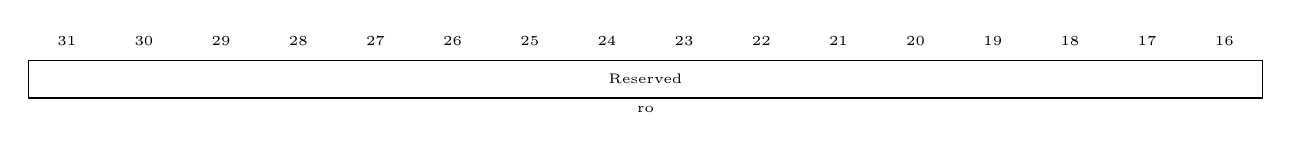
\begin{tikzpicture}[x=0.98cm,y=0.6cm]
\node[font=\tiny] at (0.5,1.2) {31};
\node[font=\tiny] at (1.5,1.2) {30};
\node[font=\tiny] at (2.5,1.2) {29};
\node[font=\tiny] at (3.5,1.2) {28};
\node[font=\tiny] at (4.5,1.2) {27};
\node[font=\tiny] at (5.5,1.2) {26};
\node[font=\tiny] at (6.5,1.2) {25};
\node[font=\tiny] at (7.5,1.2) {24};
\node[font=\tiny] at (8.5,1.2) {23};
\node[font=\tiny] at (9.5,1.2) {22};
\node[font=\tiny] at (10.5,1.2) {21};
\node[font=\tiny] at (11.5,1.2) {20};
\node[font=\tiny] at (12.5,1.2) {19};
\node[font=\tiny] at (13.5,1.2) {18};
\node[font=\tiny] at (14.5,1.2) {17};
\node[font=\tiny] at (15.5,1.2) {16};
\draw (0,0) rectangle (16,0.8);
\node[font=\tiny] at (8.0,0.4) {Reserved};
\node[font=\tiny] at (8.0,-0.25) {ro};
\end{tikzpicture}
\end{center}
\begin{center}
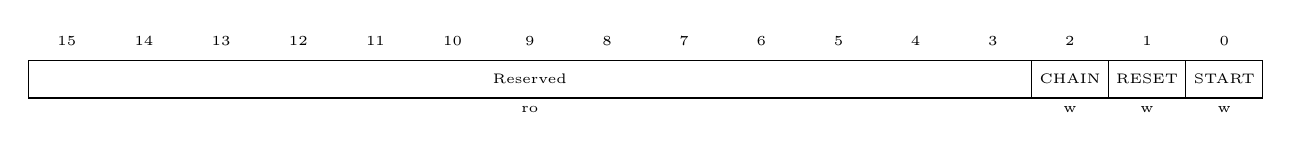
\begin{tikzpicture}[x=0.98cm,y=0.6cm]
\node[font=\tiny] at (0.5,1.2) {15};
\node[font=\tiny] at (1.5,1.2) {14};
\node[font=\tiny] at (2.5,1.2) {13};
\node[font=\tiny] at (3.5,1.2) {12};
\node[font=\tiny] at (4.5,1.2) {11};
\node[font=\tiny] at (5.5,1.2) {10};
\node[font=\tiny] at (6.5,1.2) {9};
\node[font=\tiny] at (7.5,1.2) {8};
\node[font=\tiny] at (8.5,1.2) {7};
\node[font=\tiny] at (9.5,1.2) {6};
\node[font=\tiny] at (10.5,1.2) {5};
\node[font=\tiny] at (11.5,1.2) {4};
\node[font=\tiny] at (12.5,1.2) {3};
\node[font=\tiny] at (13.5,1.2) {2};
\node[font=\tiny] at (14.5,1.2) {1};
\node[font=\tiny] at (15.5,1.2) {0};
\draw (0,0) rectangle (13,0.8);
\node[font=\tiny] at (6.5,0.4) {Reserved};
\node[font=\tiny] at (6.5,-0.25) {ro};
\draw (13,0) rectangle (14,0.8);
\node[font=\tiny] at (13.5,0.4) {CHAIN};
\node[font=\tiny] at (13.5,-0.25) {w};
\draw (14,0) rectangle (15,0.8);
\node[font=\tiny] at (14.5,0.4) {RESET};
\node[font=\tiny] at (14.5,-0.25) {w};
\draw (15,0) rectangle (16,0.8);
\node[font=\tiny] at (15.5,0.4) {START};
\node[font=\tiny] at (15.5,-0.25) {w};
\end{tikzpicture}
\end{center}
\begin{spectable}{|L{0.09}|L{0.24}|L{0.08}|L{0.15}|L{0.44}|}{Thanh ghi điều khiển}{reg:CTRL_REG}{\textbf{Bit} & \textbf{Tên} & \textbf{Kiểu} & \textbf{Giá trị mặc định} & \textbf{Mô tả}}
31:3 & Reserved & RO & 29'h0 & Đọc 0; ghi bị bỏ qua. \\\hline

2 & START\_CHAIN & W & 1'h0 & Ghi 1 yêu cầu chạy chuỗi descriptor. Khi không hỗ trợ chuỗi, tác vụ kết thúc lỗi mã 5. \\\hline

1 & SOFT\_RESET & W & 1'h0 & Ghi 1 yêu cầu soft reset; ưu tiên cao hơn cả hai lệnh START. \\\hline

0 & START & W & 1'h0 & Ghi 1 yêu cầu chạy một GEMM. Chỉ nhận khi rảnh; khi bận bỏ qua. Ghi đồng thời START và START\_CHAIN khi không có SOFT\_RESET tạo lỗi mã 1. \\\hline

\end{spectable}

\subsection{Thanh ghi trạng thái (STATUS\_REG)}
Địa chỉ offset: 0x04\par
Giá trị reset: 0x0000\_0000\par
\begin{center}
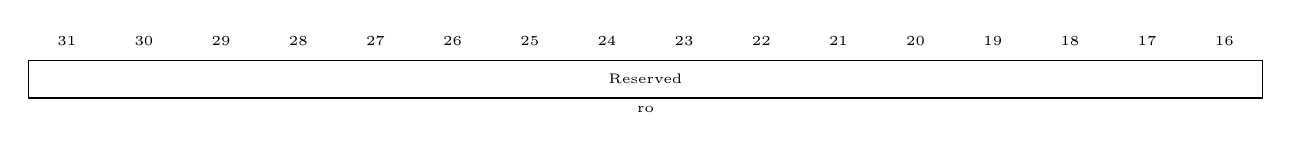
\begin{tikzpicture}[x=0.98cm,y=0.6cm]
\node[font=\tiny] at (0.5,1.2) {31};
\node[font=\tiny] at (1.5,1.2) {30};
\node[font=\tiny] at (2.5,1.2) {29};
\node[font=\tiny] at (3.5,1.2) {28};
\node[font=\tiny] at (4.5,1.2) {27};
\node[font=\tiny] at (5.5,1.2) {26};
\node[font=\tiny] at (6.5,1.2) {25};
\node[font=\tiny] at (7.5,1.2) {24};
\node[font=\tiny] at (8.5,1.2) {23};
\node[font=\tiny] at (9.5,1.2) {22};
\node[font=\tiny] at (10.5,1.2) {21};
\node[font=\tiny] at (11.5,1.2) {20};
\node[font=\tiny] at (12.5,1.2) {19};
\node[font=\tiny] at (13.5,1.2) {18};
\node[font=\tiny] at (14.5,1.2) {17};
\node[font=\tiny] at (15.5,1.2) {16};
\draw (0,0) rectangle (16,0.8);
\node[font=\tiny] at (8.0,0.4) {Reserved};
\node[font=\tiny] at (8.0,-0.25) {ro};
\end{tikzpicture}
\end{center}
\begin{center}
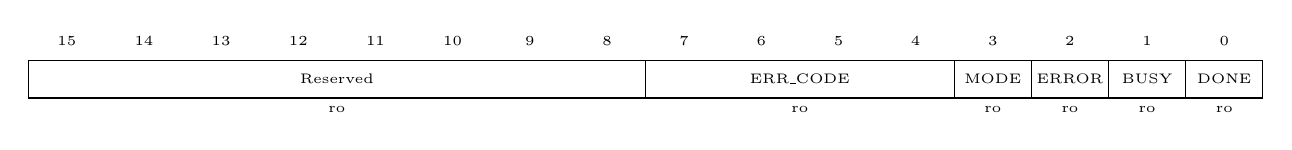
\begin{tikzpicture}[x=0.98cm,y=0.6cm]
\node[font=\tiny] at (0.5,1.2) {15};
\node[font=\tiny] at (1.5,1.2) {14};
\node[font=\tiny] at (2.5,1.2) {13};
\node[font=\tiny] at (3.5,1.2) {12};
\node[font=\tiny] at (4.5,1.2) {11};
\node[font=\tiny] at (5.5,1.2) {10};
\node[font=\tiny] at (6.5,1.2) {9};
\node[font=\tiny] at (7.5,1.2) {8};
\node[font=\tiny] at (8.5,1.2) {7};
\node[font=\tiny] at (9.5,1.2) {6};
\node[font=\tiny] at (10.5,1.2) {5};
\node[font=\tiny] at (11.5,1.2) {4};
\node[font=\tiny] at (12.5,1.2) {3};
\node[font=\tiny] at (13.5,1.2) {2};
\node[font=\tiny] at (14.5,1.2) {1};
\node[font=\tiny] at (15.5,1.2) {0};
\draw (0,0) rectangle (8,0.8);
\node[font=\tiny] at (4.0,0.4) {Reserved};
\node[font=\tiny] at (4.0,-0.25) {ro};
\draw (8,0) rectangle (12,0.8);
\node[font=\tiny] at (10.0,0.4) {ERR\_CODE};
\node[font=\tiny] at (10.0,-0.25) {ro};
\draw (12,0) rectangle (13,0.8);
\node[font=\tiny] at (12.5,0.4) {MODE};
\node[font=\tiny] at (12.5,-0.25) {ro};
\draw (13,0) rectangle (14,0.8);
\node[font=\tiny] at (13.5,0.4) {ERROR};
\node[font=\tiny] at (13.5,-0.25) {ro};
\draw (14,0) rectangle (15,0.8);
\node[font=\tiny] at (14.5,0.4) {BUSY};
\node[font=\tiny] at (14.5,-0.25) {ro};
\draw (15,0) rectangle (16,0.8);
\node[font=\tiny] at (15.5,0.4) {DONE};
\node[font=\tiny] at (15.5,-0.25) {ro};
\end{tikzpicture}
\end{center}
\begin{spectable}{|L{0.09}|L{0.24}|L{0.08}|L{0.15}|L{0.44}|}{Thanh ghi trạng thái}{reg:STATUS_REG}{\textbf{Bit} & \textbf{Tên} & \textbf{Kiểu} & \textbf{Giá trị mặc định} & \textbf{Mô tả}}
31:8 & Reserved & RO & 24'h0 & Đọc 0; ghi bị bỏ qua. \\\hline

7:4 & ERR\_CODE & RO & 4'h0 & Mã lỗi của tác vụ; bằng 0 khi ERROR = 0. Bảng mã lỗi ở dưới. \\\hline

3 & MODE & RO & 1'h0 & 0: tác vụ đơn; 1: chuỗi descriptor. Giữ chế độ tác vụ gần nhất. \\\hline

2 & ERROR & RO & 1'h0 & Cờ lỗi sticky; xóa khi nhận tác vụ mới hoặc reset. \\\hline

1 & BUSY & RO & 1'h0 & Tác vụ hoặc chuỗi soft reset đang chạy. Về 0 cùng cạnh đặt DONE hoặc ERROR. \\\hline

0 & DONE & RO & 1'h0 & Sticky; chỉ đặt khi toàn bộ kết quả đã ghi DRAM thành công. Xóa khi nhận tác vụ mới hoặc reset. \\\hline

\end{spectable}

\subsection{Kích thước ma trận (MATRIX\_DIM)}
Địa chỉ offset: 0x08\par
Giá trị reset: 0x0000\_0000\par
\begin{center}
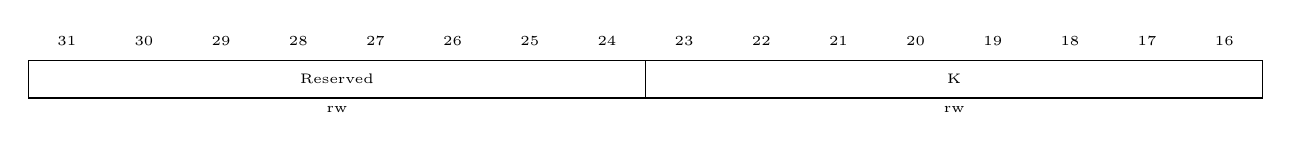
\begin{tikzpicture}[x=0.98cm,y=0.6cm]
\node[font=\tiny] at (0.5,1.2) {31};
\node[font=\tiny] at (1.5,1.2) {30};
\node[font=\tiny] at (2.5,1.2) {29};
\node[font=\tiny] at (3.5,1.2) {28};
\node[font=\tiny] at (4.5,1.2) {27};
\node[font=\tiny] at (5.5,1.2) {26};
\node[font=\tiny] at (6.5,1.2) {25};
\node[font=\tiny] at (7.5,1.2) {24};
\node[font=\tiny] at (8.5,1.2) {23};
\node[font=\tiny] at (9.5,1.2) {22};
\node[font=\tiny] at (10.5,1.2) {21};
\node[font=\tiny] at (11.5,1.2) {20};
\node[font=\tiny] at (12.5,1.2) {19};
\node[font=\tiny] at (13.5,1.2) {18};
\node[font=\tiny] at (14.5,1.2) {17};
\node[font=\tiny] at (15.5,1.2) {16};
\draw (0,0) rectangle (8,0.8);
\node[font=\tiny] at (4.0,0.4) {Reserved};
\node[font=\tiny] at (4.0,-0.25) {rw};
\draw (8,0) rectangle (16,0.8);
\node[font=\tiny] at (12.0,0.4) {K};
\node[font=\tiny] at (12.0,-0.25) {rw};
\end{tikzpicture}
\end{center}
\begin{center}
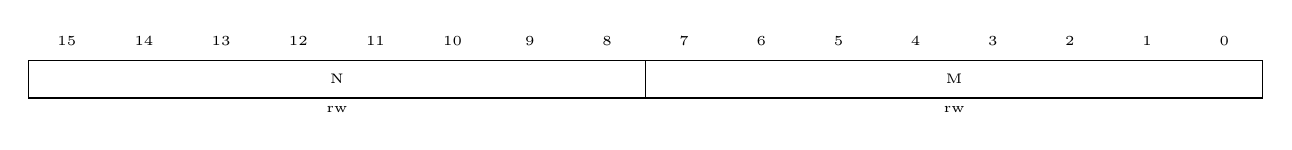
\begin{tikzpicture}[x=0.98cm,y=0.6cm]
\node[font=\tiny] at (0.5,1.2) {15};
\node[font=\tiny] at (1.5,1.2) {14};
\node[font=\tiny] at (2.5,1.2) {13};
\node[font=\tiny] at (3.5,1.2) {12};
\node[font=\tiny] at (4.5,1.2) {11};
\node[font=\tiny] at (5.5,1.2) {10};
\node[font=\tiny] at (6.5,1.2) {9};
\node[font=\tiny] at (7.5,1.2) {8};
\node[font=\tiny] at (8.5,1.2) {7};
\node[font=\tiny] at (9.5,1.2) {6};
\node[font=\tiny] at (10.5,1.2) {5};
\node[font=\tiny] at (11.5,1.2) {4};
\node[font=\tiny] at (12.5,1.2) {3};
\node[font=\tiny] at (13.5,1.2) {2};
\node[font=\tiny] at (14.5,1.2) {1};
\node[font=\tiny] at (15.5,1.2) {0};
\draw (0,0) rectangle (8,0.8);
\node[font=\tiny] at (4.0,0.4) {N};
\node[font=\tiny] at (4.0,-0.25) {rw};
\draw (8,0) rectangle (16,0.8);
\node[font=\tiny] at (12.0,0.4) {M};
\node[font=\tiny] at (12.0,-0.25) {rw};
\end{tikzpicture}
\end{center}
\begin{spectable}{|L{0.09}|L{0.24}|L{0.08}|L{0.15}|L{0.44}|}{Kích thước ma trận}{reg:MATRIX_DIM}{\textbf{Bit} & \textbf{Tên} & \textbf{Kiểu} & \textbf{Giá trị mặc định} & \textbf{Mô tả}}
31:24 & Reserved & RW & 8'h0 & Lưu và đọc lại; phải bằng 0 khi khởi chạy. \\\hline

23:16 & K & RW & 8'h0 & Số cột A/số hàng B; 4, 8, …, 32. \\\hline

15:8 & N & RW & 8'h0 & Số cột B/C; 4, 8, …, 32. \\\hline

7:0 & M & RW & 8'h0 & Số hàng A/C; 1 … 32. \\\hline

\end{spectable}

\subsection{Địa chỉ byte của A (BASE\_ADDR\_IN)}
Địa chỉ offset: 0x0C\par
Giá trị reset: 0x0000\_0000\par
\begin{center}
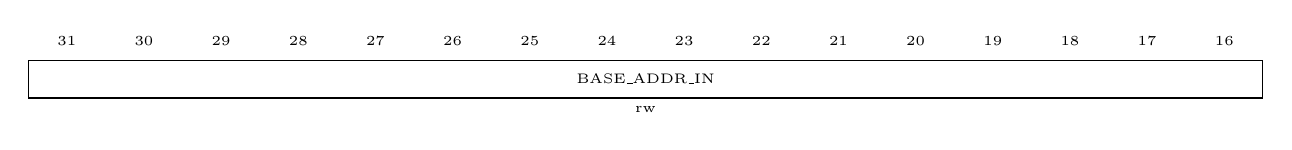
\begin{tikzpicture}[x=0.98cm,y=0.6cm]
\node[font=\tiny] at (0.5,1.2) {31};
\node[font=\tiny] at (1.5,1.2) {30};
\node[font=\tiny] at (2.5,1.2) {29};
\node[font=\tiny] at (3.5,1.2) {28};
\node[font=\tiny] at (4.5,1.2) {27};
\node[font=\tiny] at (5.5,1.2) {26};
\node[font=\tiny] at (6.5,1.2) {25};
\node[font=\tiny] at (7.5,1.2) {24};
\node[font=\tiny] at (8.5,1.2) {23};
\node[font=\tiny] at (9.5,1.2) {22};
\node[font=\tiny] at (10.5,1.2) {21};
\node[font=\tiny] at (11.5,1.2) {20};
\node[font=\tiny] at (12.5,1.2) {19};
\node[font=\tiny] at (13.5,1.2) {18};
\node[font=\tiny] at (14.5,1.2) {17};
\node[font=\tiny] at (15.5,1.2) {16};
\draw (0,0) rectangle (16,0.8);
\node[font=\tiny] at (8.0,0.4) {BASE\_ADDR\_IN};
\node[font=\tiny] at (8.0,-0.25) {rw};
\end{tikzpicture}
\end{center}
\begin{center}
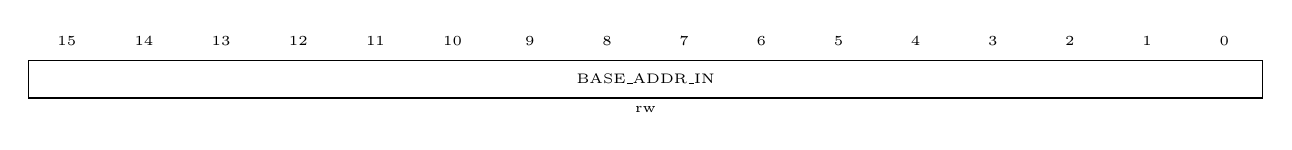
\begin{tikzpicture}[x=0.98cm,y=0.6cm]
\node[font=\tiny] at (0.5,1.2) {15};
\node[font=\tiny] at (1.5,1.2) {14};
\node[font=\tiny] at (2.5,1.2) {13};
\node[font=\tiny] at (3.5,1.2) {12};
\node[font=\tiny] at (4.5,1.2) {11};
\node[font=\tiny] at (5.5,1.2) {10};
\node[font=\tiny] at (6.5,1.2) {9};
\node[font=\tiny] at (7.5,1.2) {8};
\node[font=\tiny] at (8.5,1.2) {7};
\node[font=\tiny] at (9.5,1.2) {6};
\node[font=\tiny] at (10.5,1.2) {5};
\node[font=\tiny] at (11.5,1.2) {4};
\node[font=\tiny] at (12.5,1.2) {3};
\node[font=\tiny] at (13.5,1.2) {2};
\node[font=\tiny] at (14.5,1.2) {1};
\node[font=\tiny] at (15.5,1.2) {0};
\draw (0,0) rectangle (16,0.8);
\node[font=\tiny] at (8.0,0.4) {BASE\_ADDR\_IN};
\node[font=\tiny] at (8.0,-0.25) {rw};
\end{tikzpicture}
\end{center}
\begin{spectable}{|L{0.09}|L{0.24}|L{0.08}|L{0.15}|L{0.44}|}{Địa chỉ byte của A}{reg:BASE_ADDR_IN}{\textbf{Bit} & \textbf{Tên} & \textbf{Kiểu} & \textbf{Giá trị mặc định} & \textbf{Mô tả}}
31:0 & BASE\_ADDR\_IN & RW & 32'h0 & Địa chỉ byte của A; căn 4 byte khi được sử dụng. \\\hline

\end{spectable}

\subsection{Địa chỉ byte của B (BASE\_ADDR\_WEIGHT)}
Địa chỉ offset: 0x10\par
Giá trị reset: 0x0000\_0000\par
\begin{center}
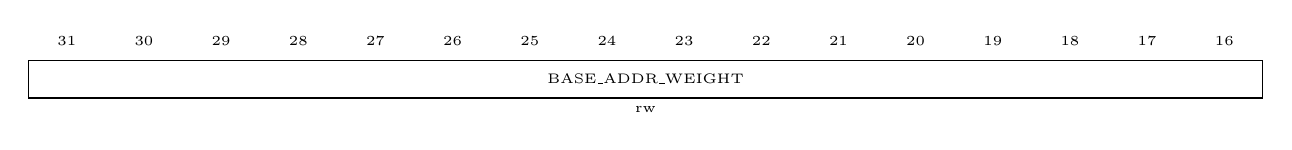
\begin{tikzpicture}[x=0.98cm,y=0.6cm]
\node[font=\tiny] at (0.5,1.2) {31};
\node[font=\tiny] at (1.5,1.2) {30};
\node[font=\tiny] at (2.5,1.2) {29};
\node[font=\tiny] at (3.5,1.2) {28};
\node[font=\tiny] at (4.5,1.2) {27};
\node[font=\tiny] at (5.5,1.2) {26};
\node[font=\tiny] at (6.5,1.2) {25};
\node[font=\tiny] at (7.5,1.2) {24};
\node[font=\tiny] at (8.5,1.2) {23};
\node[font=\tiny] at (9.5,1.2) {22};
\node[font=\tiny] at (10.5,1.2) {21};
\node[font=\tiny] at (11.5,1.2) {20};
\node[font=\tiny] at (12.5,1.2) {19};
\node[font=\tiny] at (13.5,1.2) {18};
\node[font=\tiny] at (14.5,1.2) {17};
\node[font=\tiny] at (15.5,1.2) {16};
\draw (0,0) rectangle (16,0.8);
\node[font=\tiny] at (8.0,0.4) {BASE\_ADDR\_WEIGHT};
\node[font=\tiny] at (8.0,-0.25) {rw};
\end{tikzpicture}
\end{center}
\begin{center}
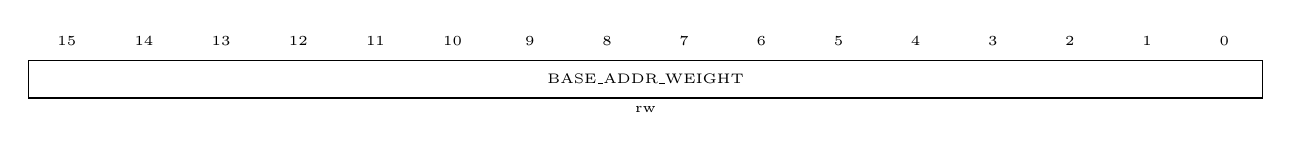
\begin{tikzpicture}[x=0.98cm,y=0.6cm]
\node[font=\tiny] at (0.5,1.2) {15};
\node[font=\tiny] at (1.5,1.2) {14};
\node[font=\tiny] at (2.5,1.2) {13};
\node[font=\tiny] at (3.5,1.2) {12};
\node[font=\tiny] at (4.5,1.2) {11};
\node[font=\tiny] at (5.5,1.2) {10};
\node[font=\tiny] at (6.5,1.2) {9};
\node[font=\tiny] at (7.5,1.2) {8};
\node[font=\tiny] at (8.5,1.2) {7};
\node[font=\tiny] at (9.5,1.2) {6};
\node[font=\tiny] at (10.5,1.2) {5};
\node[font=\tiny] at (11.5,1.2) {4};
\node[font=\tiny] at (12.5,1.2) {3};
\node[font=\tiny] at (13.5,1.2) {2};
\node[font=\tiny] at (14.5,1.2) {1};
\node[font=\tiny] at (15.5,1.2) {0};
\draw (0,0) rectangle (16,0.8);
\node[font=\tiny] at (8.0,0.4) {BASE\_ADDR\_WEIGHT};
\node[font=\tiny] at (8.0,-0.25) {rw};
\end{tikzpicture}
\end{center}
\begin{spectable}{|L{0.09}|L{0.24}|L{0.08}|L{0.15}|L{0.44}|}{Địa chỉ byte của B}{reg:BASE_ADDR_WEIGHT}{\textbf{Bit} & \textbf{Tên} & \textbf{Kiểu} & \textbf{Giá trị mặc định} & \textbf{Mô tả}}
31:0 & BASE\_ADDR\_WEIGHT & RW & 32'h0 & Địa chỉ byte của B; căn 4 byte khi được sử dụng. \\\hline

\end{spectable}

\subsection{Địa chỉ byte vùng kết quả C hoặc Y (BASE\_ADDR\_OUT)}
Địa chỉ offset: 0x14\par
Giá trị reset: 0x0000\_0000\par
\begin{center}
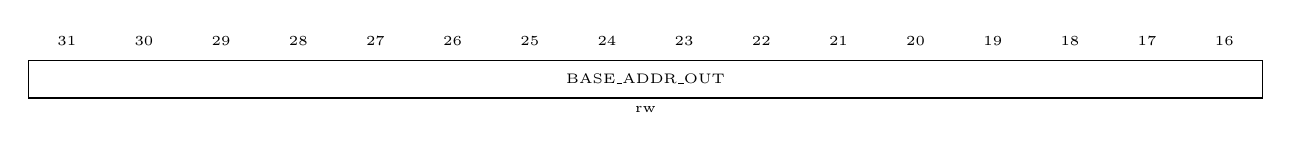
\begin{tikzpicture}[x=0.98cm,y=0.6cm]
\node[font=\tiny] at (0.5,1.2) {31};
\node[font=\tiny] at (1.5,1.2) {30};
\node[font=\tiny] at (2.5,1.2) {29};
\node[font=\tiny] at (3.5,1.2) {28};
\node[font=\tiny] at (4.5,1.2) {27};
\node[font=\tiny] at (5.5,1.2) {26};
\node[font=\tiny] at (6.5,1.2) {25};
\node[font=\tiny] at (7.5,1.2) {24};
\node[font=\tiny] at (8.5,1.2) {23};
\node[font=\tiny] at (9.5,1.2) {22};
\node[font=\tiny] at (10.5,1.2) {21};
\node[font=\tiny] at (11.5,1.2) {20};
\node[font=\tiny] at (12.5,1.2) {19};
\node[font=\tiny] at (13.5,1.2) {18};
\node[font=\tiny] at (14.5,1.2) {17};
\node[font=\tiny] at (15.5,1.2) {16};
\draw (0,0) rectangle (16,0.8);
\node[font=\tiny] at (8.0,0.4) {BASE\_ADDR\_OUT};
\node[font=\tiny] at (8.0,-0.25) {rw};
\end{tikzpicture}
\end{center}
\begin{center}
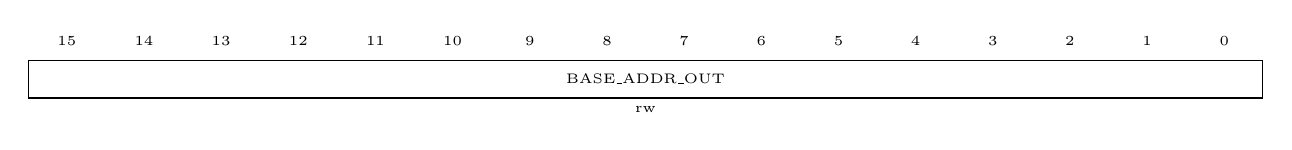
\begin{tikzpicture}[x=0.98cm,y=0.6cm]
\node[font=\tiny] at (0.5,1.2) {15};
\node[font=\tiny] at (1.5,1.2) {14};
\node[font=\tiny] at (2.5,1.2) {13};
\node[font=\tiny] at (3.5,1.2) {12};
\node[font=\tiny] at (4.5,1.2) {11};
\node[font=\tiny] at (5.5,1.2) {10};
\node[font=\tiny] at (6.5,1.2) {9};
\node[font=\tiny] at (7.5,1.2) {8};
\node[font=\tiny] at (8.5,1.2) {7};
\node[font=\tiny] at (9.5,1.2) {6};
\node[font=\tiny] at (10.5,1.2) {5};
\node[font=\tiny] at (11.5,1.2) {4};
\node[font=\tiny] at (12.5,1.2) {3};
\node[font=\tiny] at (13.5,1.2) {2};
\node[font=\tiny] at (14.5,1.2) {1};
\node[font=\tiny] at (15.5,1.2) {0};
\draw (0,0) rectangle (16,0.8);
\node[font=\tiny] at (8.0,0.4) {BASE\_ADDR\_OUT};
\node[font=\tiny] at (8.0,-0.25) {rw};
\end{tikzpicture}
\end{center}
\begin{spectable}{|L{0.09}|L{0.24}|L{0.08}|L{0.15}|L{0.44}|}{Địa chỉ byte vùng kết quả C hoặc Y}{reg:BASE_ADDR_OUT}{\textbf{Bit} & \textbf{Tên} & \textbf{Kiểu} & \textbf{Giá trị mặc định} & \textbf{Mô tả}}
31:0 & BASE\_ADDR\_OUT & RW & 32'h0 & Địa chỉ byte vùng kết quả C hoặc Y; căn 4 byte khi được sử dụng. \\\hline

\end{spectable}

\subsection{Điều khiển hậu xử lý (POST\_CTRL)}
Địa chỉ offset: 0x18\par
Giá trị reset: 0x0000\_0000\par
\begin{center}
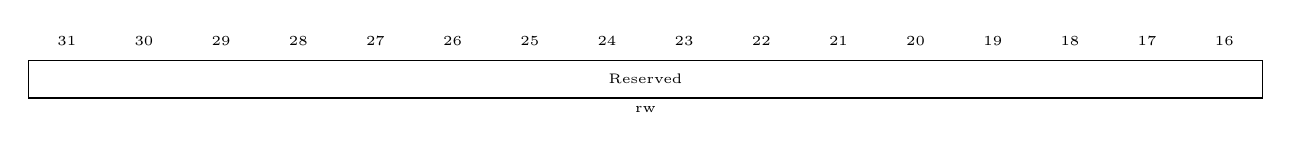
\begin{tikzpicture}[x=0.98cm,y=0.6cm]
\node[font=\tiny] at (0.5,1.2) {31};
\node[font=\tiny] at (1.5,1.2) {30};
\node[font=\tiny] at (2.5,1.2) {29};
\node[font=\tiny] at (3.5,1.2) {28};
\node[font=\tiny] at (4.5,1.2) {27};
\node[font=\tiny] at (5.5,1.2) {26};
\node[font=\tiny] at (6.5,1.2) {25};
\node[font=\tiny] at (7.5,1.2) {24};
\node[font=\tiny] at (8.5,1.2) {23};
\node[font=\tiny] at (9.5,1.2) {22};
\node[font=\tiny] at (10.5,1.2) {21};
\node[font=\tiny] at (11.5,1.2) {20};
\node[font=\tiny] at (12.5,1.2) {19};
\node[font=\tiny] at (13.5,1.2) {18};
\node[font=\tiny] at (14.5,1.2) {17};
\node[font=\tiny] at (15.5,1.2) {16};
\draw (0,0) rectangle (16,0.8);
\node[font=\tiny] at (8.0,0.4) {Reserved};
\node[font=\tiny] at (8.0,-0.25) {rw};
\end{tikzpicture}
\end{center}
\begin{center}
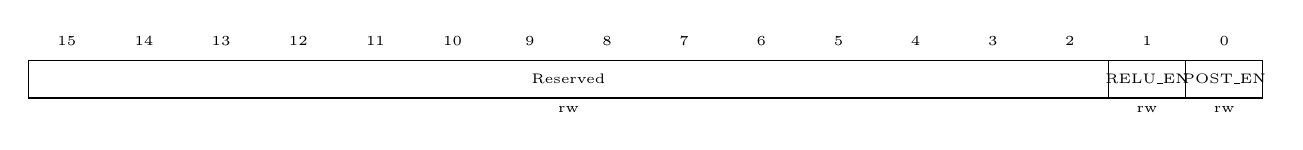
\begin{tikzpicture}[x=0.98cm,y=0.6cm]
\node[font=\tiny] at (0.5,1.2) {15};
\node[font=\tiny] at (1.5,1.2) {14};
\node[font=\tiny] at (2.5,1.2) {13};
\node[font=\tiny] at (3.5,1.2) {12};
\node[font=\tiny] at (4.5,1.2) {11};
\node[font=\tiny] at (5.5,1.2) {10};
\node[font=\tiny] at (6.5,1.2) {9};
\node[font=\tiny] at (7.5,1.2) {8};
\node[font=\tiny] at (8.5,1.2) {7};
\node[font=\tiny] at (9.5,1.2) {6};
\node[font=\tiny] at (10.5,1.2) {5};
\node[font=\tiny] at (11.5,1.2) {4};
\node[font=\tiny] at (12.5,1.2) {3};
\node[font=\tiny] at (13.5,1.2) {2};
\node[font=\tiny] at (14.5,1.2) {1};
\node[font=\tiny] at (15.5,1.2) {0};
\draw (0,0) rectangle (14,0.8);
\node[font=\tiny] at (7.0,0.4) {Reserved};
\node[font=\tiny] at (7.0,-0.25) {rw};
\draw (14,0) rectangle (15,0.8);
\node[font=\tiny] at (14.5,0.4) {RELU\_EN};
\node[font=\tiny] at (14.5,-0.25) {rw};
\draw (15,0) rectangle (16,0.8);
\node[font=\tiny] at (15.5,0.4) {POST\_EN};
\node[font=\tiny] at (15.5,-0.25) {rw};
\end{tikzpicture}
\end{center}
\begin{spectable}{|L{0.09}|L{0.24}|L{0.08}|L{0.15}|L{0.44}|}{Điều khiển hậu xử lý}{reg:POST_CTRL}{\textbf{Bit} & \textbf{Tên} & \textbf{Kiểu} & \textbf{Giá trị mặc định} & \textbf{Mô tả}}
31:2 & Reserved & RW & 30'h0 & Lưu và đọc lại; phải bằng 0 khi khởi chạy. \\\hline

1 & RELU\_EN & RW & 1'h0 & Bật ReLU; chỉ hợp lệ khi POST\_EN = 1. \\\hline

0 & POST\_EN & RW & 1'h0 & 0: kết quả INT32. 1: cộng bias, requantize, tùy chọn ReLU và kẹp về INT8. \\\hline

\end{spectable}

\subsection{Địa chỉ byte vector bias; bỏ qua khi POST\_EN = 0 (BIAS\_ADDR)}
Địa chỉ offset: 0x1C\par
Giá trị reset: 0x0000\_0000\par
\begin{center}
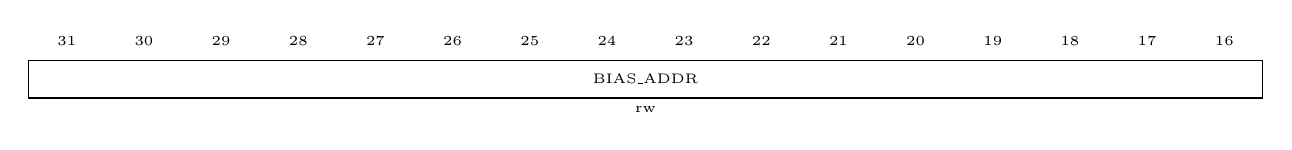
\begin{tikzpicture}[x=0.98cm,y=0.6cm]
\node[font=\tiny] at (0.5,1.2) {31};
\node[font=\tiny] at (1.5,1.2) {30};
\node[font=\tiny] at (2.5,1.2) {29};
\node[font=\tiny] at (3.5,1.2) {28};
\node[font=\tiny] at (4.5,1.2) {27};
\node[font=\tiny] at (5.5,1.2) {26};
\node[font=\tiny] at (6.5,1.2) {25};
\node[font=\tiny] at (7.5,1.2) {24};
\node[font=\tiny] at (8.5,1.2) {23};
\node[font=\tiny] at (9.5,1.2) {22};
\node[font=\tiny] at (10.5,1.2) {21};
\node[font=\tiny] at (11.5,1.2) {20};
\node[font=\tiny] at (12.5,1.2) {19};
\node[font=\tiny] at (13.5,1.2) {18};
\node[font=\tiny] at (14.5,1.2) {17};
\node[font=\tiny] at (15.5,1.2) {16};
\draw (0,0) rectangle (16,0.8);
\node[font=\tiny] at (8.0,0.4) {BIAS\_ADDR};
\node[font=\tiny] at (8.0,-0.25) {rw};
\end{tikzpicture}
\end{center}
\begin{center}
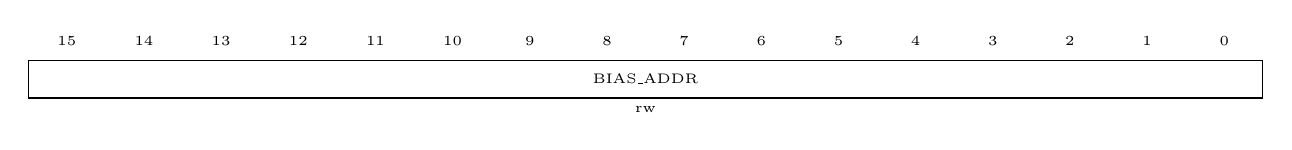
\begin{tikzpicture}[x=0.98cm,y=0.6cm]
\node[font=\tiny] at (0.5,1.2) {15};
\node[font=\tiny] at (1.5,1.2) {14};
\node[font=\tiny] at (2.5,1.2) {13};
\node[font=\tiny] at (3.5,1.2) {12};
\node[font=\tiny] at (4.5,1.2) {11};
\node[font=\tiny] at (5.5,1.2) {10};
\node[font=\tiny] at (6.5,1.2) {9};
\node[font=\tiny] at (7.5,1.2) {8};
\node[font=\tiny] at (8.5,1.2) {7};
\node[font=\tiny] at (9.5,1.2) {6};
\node[font=\tiny] at (10.5,1.2) {5};
\node[font=\tiny] at (11.5,1.2) {4};
\node[font=\tiny] at (12.5,1.2) {3};
\node[font=\tiny] at (13.5,1.2) {2};
\node[font=\tiny] at (14.5,1.2) {1};
\node[font=\tiny] at (15.5,1.2) {0};
\draw (0,0) rectangle (16,0.8);
\node[font=\tiny] at (8.0,0.4) {BIAS\_ADDR};
\node[font=\tiny] at (8.0,-0.25) {rw};
\end{tikzpicture}
\end{center}
\begin{spectable}{|L{0.09}|L{0.24}|L{0.08}|L{0.15}|L{0.44}|}{Địa chỉ byte vector bias; bỏ qua khi POST\_EN = 0}{reg:BIAS_ADDR}{\textbf{Bit} & \textbf{Tên} & \textbf{Kiểu} & \textbf{Giá trị mặc định} & \textbf{Mô tả}}
31:0 & BIAS\_ADDR & RW & 32'h0 & Địa chỉ byte vector bias; bỏ qua khi POST\_EN = 0; căn 4 byte khi được sử dụng. \\\hline

\end{spectable}

\subsection{Hệ số lượng tử (QUANT\_M0)}
Địa chỉ offset: 0x20\par
Giá trị reset: 0x0000\_0000\par
\begin{center}
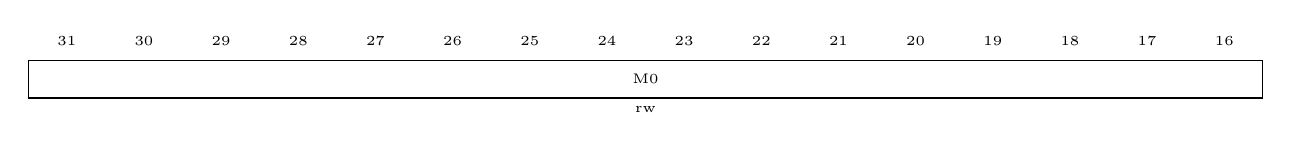
\begin{tikzpicture}[x=0.98cm,y=0.6cm]
\node[font=\tiny] at (0.5,1.2) {31};
\node[font=\tiny] at (1.5,1.2) {30};
\node[font=\tiny] at (2.5,1.2) {29};
\node[font=\tiny] at (3.5,1.2) {28};
\node[font=\tiny] at (4.5,1.2) {27};
\node[font=\tiny] at (5.5,1.2) {26};
\node[font=\tiny] at (6.5,1.2) {25};
\node[font=\tiny] at (7.5,1.2) {24};
\node[font=\tiny] at (8.5,1.2) {23};
\node[font=\tiny] at (9.5,1.2) {22};
\node[font=\tiny] at (10.5,1.2) {21};
\node[font=\tiny] at (11.5,1.2) {20};
\node[font=\tiny] at (12.5,1.2) {19};
\node[font=\tiny] at (13.5,1.2) {18};
\node[font=\tiny] at (14.5,1.2) {17};
\node[font=\tiny] at (15.5,1.2) {16};
\draw (0,0) rectangle (16,0.8);
\node[font=\tiny] at (8.0,0.4) {M0};
\node[font=\tiny] at (8.0,-0.25) {rw};
\end{tikzpicture}
\end{center}
\begin{center}
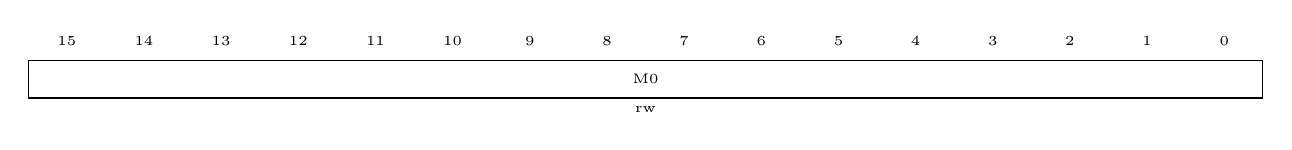
\begin{tikzpicture}[x=0.98cm,y=0.6cm]
\node[font=\tiny] at (0.5,1.2) {15};
\node[font=\tiny] at (1.5,1.2) {14};
\node[font=\tiny] at (2.5,1.2) {13};
\node[font=\tiny] at (3.5,1.2) {12};
\node[font=\tiny] at (4.5,1.2) {11};
\node[font=\tiny] at (5.5,1.2) {10};
\node[font=\tiny] at (6.5,1.2) {9};
\node[font=\tiny] at (7.5,1.2) {8};
\node[font=\tiny] at (8.5,1.2) {7};
\node[font=\tiny] at (9.5,1.2) {6};
\node[font=\tiny] at (10.5,1.2) {5};
\node[font=\tiny] at (11.5,1.2) {4};
\node[font=\tiny] at (12.5,1.2) {3};
\node[font=\tiny] at (13.5,1.2) {2};
\node[font=\tiny] at (14.5,1.2) {1};
\node[font=\tiny] at (15.5,1.2) {0};
\draw (0,0) rectangle (16,0.8);
\node[font=\tiny] at (8.0,0.4) {M0};
\node[font=\tiny] at (8.0,-0.25) {rw};
\end{tikzpicture}
\end{center}
\begin{spectable}{|L{0.09}|L{0.24}|L{0.08}|L{0.15}|L{0.44}|}{Hệ số lượng tử}{reg:QUANT_M0}{\textbf{Bit} & \textbf{Tên} & \textbf{Kiểu} & \textbf{Giá trị mặc định} & \textbf{Mô tả}}
31:0 & M0 & RW & 32'h0 & Số nguyên có dấu INT32, mọi giá trị hợp lệ; bỏ qua khi POST\_EN = 0. \\\hline

\end{spectable}

\subsection{Lượng dịch lượng tử (QUANT\_SHIFT)}
Địa chỉ offset: 0x24\par
Giá trị reset: 0x0000\_0000\par
\begin{center}
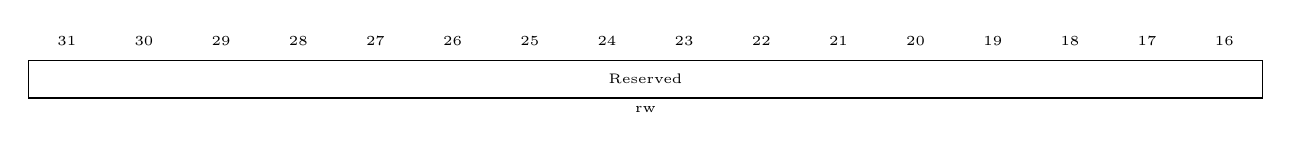
\begin{tikzpicture}[x=0.98cm,y=0.6cm]
\node[font=\tiny] at (0.5,1.2) {31};
\node[font=\tiny] at (1.5,1.2) {30};
\node[font=\tiny] at (2.5,1.2) {29};
\node[font=\tiny] at (3.5,1.2) {28};
\node[font=\tiny] at (4.5,1.2) {27};
\node[font=\tiny] at (5.5,1.2) {26};
\node[font=\tiny] at (6.5,1.2) {25};
\node[font=\tiny] at (7.5,1.2) {24};
\node[font=\tiny] at (8.5,1.2) {23};
\node[font=\tiny] at (9.5,1.2) {22};
\node[font=\tiny] at (10.5,1.2) {21};
\node[font=\tiny] at (11.5,1.2) {20};
\node[font=\tiny] at (12.5,1.2) {19};
\node[font=\tiny] at (13.5,1.2) {18};
\node[font=\tiny] at (14.5,1.2) {17};
\node[font=\tiny] at (15.5,1.2) {16};
\draw (0,0) rectangle (16,0.8);
\node[font=\tiny] at (8.0,0.4) {Reserved};
\node[font=\tiny] at (8.0,-0.25) {rw};
\end{tikzpicture}
\end{center}
\begin{center}
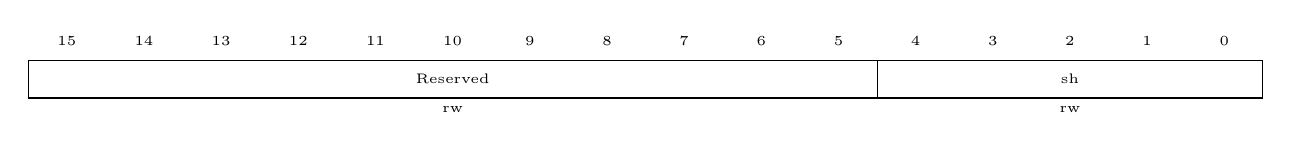
\begin{tikzpicture}[x=0.98cm,y=0.6cm]
\node[font=\tiny] at (0.5,1.2) {15};
\node[font=\tiny] at (1.5,1.2) {14};
\node[font=\tiny] at (2.5,1.2) {13};
\node[font=\tiny] at (3.5,1.2) {12};
\node[font=\tiny] at (4.5,1.2) {11};
\node[font=\tiny] at (5.5,1.2) {10};
\node[font=\tiny] at (6.5,1.2) {9};
\node[font=\tiny] at (7.5,1.2) {8};
\node[font=\tiny] at (8.5,1.2) {7};
\node[font=\tiny] at (9.5,1.2) {6};
\node[font=\tiny] at (10.5,1.2) {5};
\node[font=\tiny] at (11.5,1.2) {4};
\node[font=\tiny] at (12.5,1.2) {3};
\node[font=\tiny] at (13.5,1.2) {2};
\node[font=\tiny] at (14.5,1.2) {1};
\node[font=\tiny] at (15.5,1.2) {0};
\draw (0,0) rectangle (11,0.8);
\node[font=\tiny] at (5.5,0.4) {Reserved};
\node[font=\tiny] at (5.5,-0.25) {rw};
\draw (11,0) rectangle (16,0.8);
\node[font=\tiny] at (13.5,0.4) {sh};
\node[font=\tiny] at (13.5,-0.25) {rw};
\end{tikzpicture}
\end{center}
\begin{spectable}{|L{0.09}|L{0.24}|L{0.08}|L{0.15}|L{0.44}|}{Lượng dịch lượng tử}{reg:QUANT_SHIFT}{\textbf{Bit} & \textbf{Tên} & \textbf{Kiểu} & \textbf{Giá trị mặc định} & \textbf{Mô tả}}
31:5 & Reserved & RW & 27'h0 & Lưu và đọc lại; phải bằng 0 khi POST\_EN = 1. \\\hline

4:0 & sh & RW & 5'h0 & Số không dấu 0 … 31; tổng lượng dịch là 31 + sh. \\\hline

\end{spectable}

\subsection{Cấu hình phần cứng (HW\_CONFIG)}
Địa chỉ offset: 0x28\par
Giá trị reset: \{8\texttt{\char39}h10, 6\texttt{\char39}b0, HAS\_PINGPONG, HAS\_CHAIN, 8\texttt{\char39}d32, P[7:0]\}\par
\begin{center}
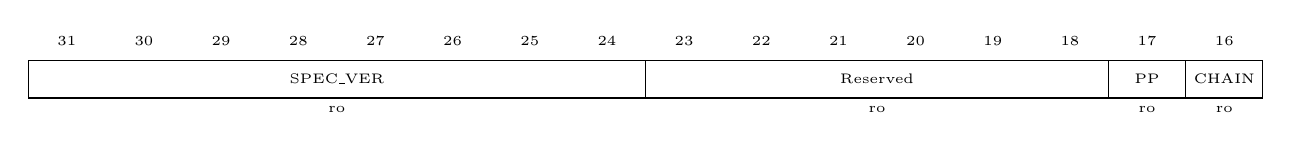
\begin{tikzpicture}[x=0.98cm,y=0.6cm]
\node[font=\tiny] at (0.5,1.2) {31};
\node[font=\tiny] at (1.5,1.2) {30};
\node[font=\tiny] at (2.5,1.2) {29};
\node[font=\tiny] at (3.5,1.2) {28};
\node[font=\tiny] at (4.5,1.2) {27};
\node[font=\tiny] at (5.5,1.2) {26};
\node[font=\tiny] at (6.5,1.2) {25};
\node[font=\tiny] at (7.5,1.2) {24};
\node[font=\tiny] at (8.5,1.2) {23};
\node[font=\tiny] at (9.5,1.2) {22};
\node[font=\tiny] at (10.5,1.2) {21};
\node[font=\tiny] at (11.5,1.2) {20};
\node[font=\tiny] at (12.5,1.2) {19};
\node[font=\tiny] at (13.5,1.2) {18};
\node[font=\tiny] at (14.5,1.2) {17};
\node[font=\tiny] at (15.5,1.2) {16};
\draw (0,0) rectangle (8,0.8);
\node[font=\tiny] at (4.0,0.4) {SPEC\_VER};
\node[font=\tiny] at (4.0,-0.25) {ro};
\draw (8,0) rectangle (14,0.8);
\node[font=\tiny] at (11.0,0.4) {Reserved};
\node[font=\tiny] at (11.0,-0.25) {ro};
\draw (14,0) rectangle (15,0.8);
\node[font=\tiny] at (14.5,0.4) {PP};
\node[font=\tiny] at (14.5,-0.25) {ro};
\draw (15,0) rectangle (16,0.8);
\node[font=\tiny] at (15.5,0.4) {CHAIN};
\node[font=\tiny] at (15.5,-0.25) {ro};
\end{tikzpicture}
\end{center}
\begin{center}
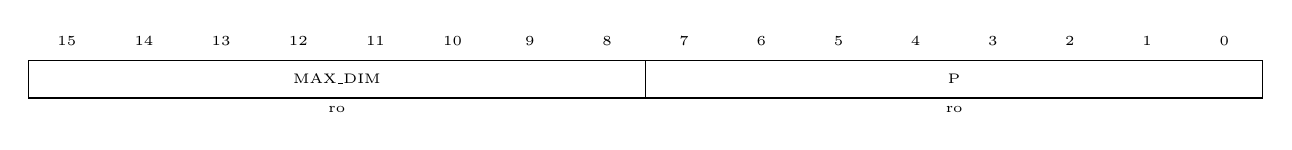
\begin{tikzpicture}[x=0.98cm,y=0.6cm]
\node[font=\tiny] at (0.5,1.2) {15};
\node[font=\tiny] at (1.5,1.2) {14};
\node[font=\tiny] at (2.5,1.2) {13};
\node[font=\tiny] at (3.5,1.2) {12};
\node[font=\tiny] at (4.5,1.2) {11};
\node[font=\tiny] at (5.5,1.2) {10};
\node[font=\tiny] at (6.5,1.2) {9};
\node[font=\tiny] at (7.5,1.2) {8};
\node[font=\tiny] at (8.5,1.2) {7};
\node[font=\tiny] at (9.5,1.2) {6};
\node[font=\tiny] at (10.5,1.2) {5};
\node[font=\tiny] at (11.5,1.2) {4};
\node[font=\tiny] at (12.5,1.2) {3};
\node[font=\tiny] at (13.5,1.2) {2};
\node[font=\tiny] at (14.5,1.2) {1};
\node[font=\tiny] at (15.5,1.2) {0};
\draw (0,0) rectangle (8,0.8);
\node[font=\tiny] at (4.0,0.4) {MAX\_DIM};
\node[font=\tiny] at (4.0,-0.25) {ro};
\draw (8,0) rectangle (16,0.8);
\node[font=\tiny] at (12.0,0.4) {P};
\node[font=\tiny] at (12.0,-0.25) {ro};
\end{tikzpicture}
\end{center}
\begin{spectable}{|L{0.09}|L{0.24}|L{0.08}|L{0.15}|L{0.44}|}{Cấu hình phần cứng}{reg:HW_CONFIG}{\textbf{Bit} & \textbf{Tên} & \textbf{Kiểu} & \textbf{Giá trị mặc định} & \textbf{Mô tả}}
31:24 & SPEC\_VER & RO & 0x10 & Phiên bản giao diện phần cứng v1.0; việc biên tập tài liệu không thay đổi giá trị này. \\\hline

23:18 & Reserved & RO & 6'h0 & Đọc 0; ghi bị bỏ qua. \\\hline

17 & HAS\_PINGPONG & RO & tham số & Có hai bank mỗi buffer. \\\hline

16 & HAS\_CHAIN & RO & tham số & Có chế độ chuỗi descriptor. \\\hline

15:8 & MAX\_DIM & RO & 32 & Kích thước ma trận tối đa. \\\hline

7:0 & P & RO & tham số & Kích thước array; 4 hoặc 8. \\\hline

\end{spectable}

\subsection{Tổng số chu kỳ BUSY của tác vụ (PERF\_TOTAL)}
Địa chỉ offset: 0x2C\par
Giá trị reset: 0x0000\_0000\par
\begin{center}
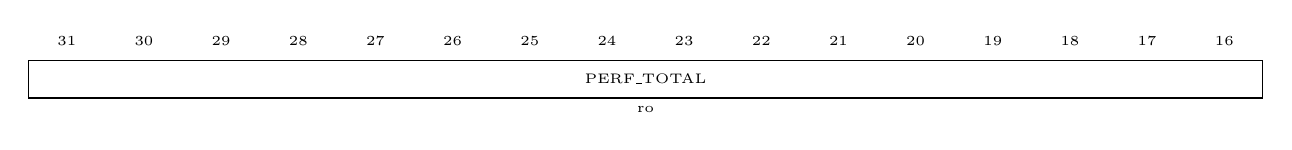
\begin{tikzpicture}[x=0.98cm,y=0.6cm]
\node[font=\tiny] at (0.5,1.2) {31};
\node[font=\tiny] at (1.5,1.2) {30};
\node[font=\tiny] at (2.5,1.2) {29};
\node[font=\tiny] at (3.5,1.2) {28};
\node[font=\tiny] at (4.5,1.2) {27};
\node[font=\tiny] at (5.5,1.2) {26};
\node[font=\tiny] at (6.5,1.2) {25};
\node[font=\tiny] at (7.5,1.2) {24};
\node[font=\tiny] at (8.5,1.2) {23};
\node[font=\tiny] at (9.5,1.2) {22};
\node[font=\tiny] at (10.5,1.2) {21};
\node[font=\tiny] at (11.5,1.2) {20};
\node[font=\tiny] at (12.5,1.2) {19};
\node[font=\tiny] at (13.5,1.2) {18};
\node[font=\tiny] at (14.5,1.2) {17};
\node[font=\tiny] at (15.5,1.2) {16};
\draw (0,0) rectangle (16,0.8);
\node[font=\tiny] at (8.0,0.4) {PERF\_TOTAL};
\node[font=\tiny] at (8.0,-0.25) {ro};
\end{tikzpicture}
\end{center}
\begin{center}
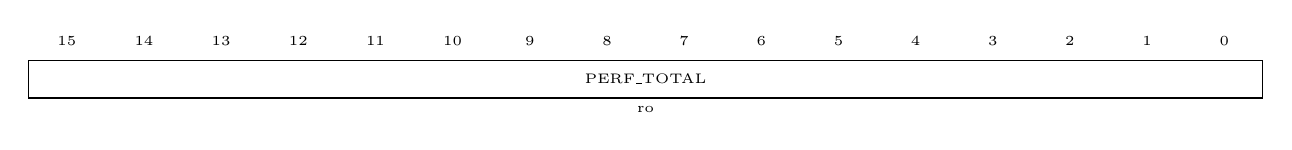
\begin{tikzpicture}[x=0.98cm,y=0.6cm]
\node[font=\tiny] at (0.5,1.2) {15};
\node[font=\tiny] at (1.5,1.2) {14};
\node[font=\tiny] at (2.5,1.2) {13};
\node[font=\tiny] at (3.5,1.2) {12};
\node[font=\tiny] at (4.5,1.2) {11};
\node[font=\tiny] at (5.5,1.2) {10};
\node[font=\tiny] at (6.5,1.2) {9};
\node[font=\tiny] at (7.5,1.2) {8};
\node[font=\tiny] at (8.5,1.2) {7};
\node[font=\tiny] at (9.5,1.2) {6};
\node[font=\tiny] at (10.5,1.2) {5};
\node[font=\tiny] at (11.5,1.2) {4};
\node[font=\tiny] at (12.5,1.2) {3};
\node[font=\tiny] at (13.5,1.2) {2};
\node[font=\tiny] at (14.5,1.2) {1};
\node[font=\tiny] at (15.5,1.2) {0};
\draw (0,0) rectangle (16,0.8);
\node[font=\tiny] at (8.0,0.4) {PERF\_TOTAL};
\node[font=\tiny] at (8.0,-0.25) {ro};
\end{tikzpicture}
\end{center}
\begin{spectable}{|L{0.09}|L{0.24}|L{0.08}|L{0.15}|L{0.44}|}{Tổng số chu kỳ BUSY của tác vụ}{reg:PERF_TOTAL}{\textbf{Bit} & \textbf{Tên} & \textbf{Kiểu} & \textbf{Giá trị mặc định} & \textbf{Mô tả}}
31:0 & PERF\_TOTAL & RO & 32'h0 & Tổng số chu kỳ BUSY của tác vụ. Xóa khi nhận tác vụ hoặc reset; bão hòa tại 0xFFFF\_FFFF, giữ sau khi kết thúc. \\\hline

\end{spectable}

\subsection{Số chu kỳ LOAD, không tính FETCH (PERF\_LOAD)}
Địa chỉ offset: 0x30\par
Giá trị reset: 0x0000\_0000\par
\begin{center}
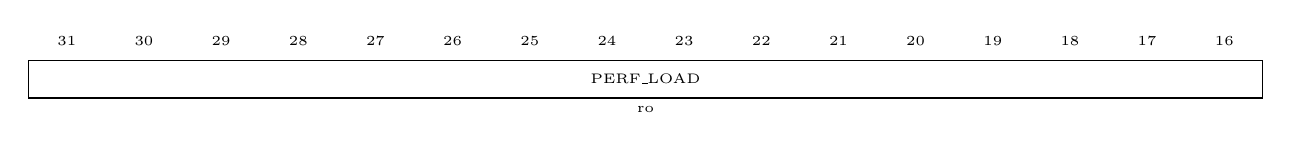
\begin{tikzpicture}[x=0.98cm,y=0.6cm]
\node[font=\tiny] at (0.5,1.2) {31};
\node[font=\tiny] at (1.5,1.2) {30};
\node[font=\tiny] at (2.5,1.2) {29};
\node[font=\tiny] at (3.5,1.2) {28};
\node[font=\tiny] at (4.5,1.2) {27};
\node[font=\tiny] at (5.5,1.2) {26};
\node[font=\tiny] at (6.5,1.2) {25};
\node[font=\tiny] at (7.5,1.2) {24};
\node[font=\tiny] at (8.5,1.2) {23};
\node[font=\tiny] at (9.5,1.2) {22};
\node[font=\tiny] at (10.5,1.2) {21};
\node[font=\tiny] at (11.5,1.2) {20};
\node[font=\tiny] at (12.5,1.2) {19};
\node[font=\tiny] at (13.5,1.2) {18};
\node[font=\tiny] at (14.5,1.2) {17};
\node[font=\tiny] at (15.5,1.2) {16};
\draw (0,0) rectangle (16,0.8);
\node[font=\tiny] at (8.0,0.4) {PERF\_LOAD};
\node[font=\tiny] at (8.0,-0.25) {ro};
\end{tikzpicture}
\end{center}
\begin{center}
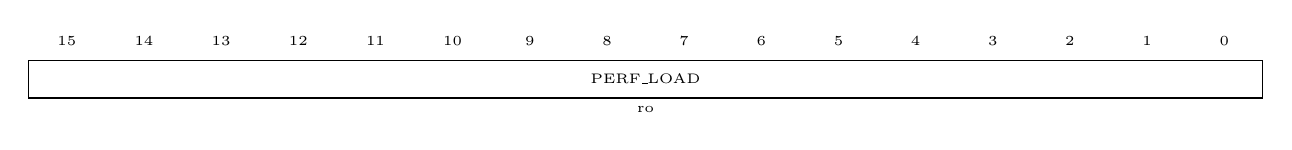
\begin{tikzpicture}[x=0.98cm,y=0.6cm]
\node[font=\tiny] at (0.5,1.2) {15};
\node[font=\tiny] at (1.5,1.2) {14};
\node[font=\tiny] at (2.5,1.2) {13};
\node[font=\tiny] at (3.5,1.2) {12};
\node[font=\tiny] at (4.5,1.2) {11};
\node[font=\tiny] at (5.5,1.2) {10};
\node[font=\tiny] at (6.5,1.2) {9};
\node[font=\tiny] at (7.5,1.2) {8};
\node[font=\tiny] at (8.5,1.2) {7};
\node[font=\tiny] at (9.5,1.2) {6};
\node[font=\tiny] at (10.5,1.2) {5};
\node[font=\tiny] at (11.5,1.2) {4};
\node[font=\tiny] at (12.5,1.2) {3};
\node[font=\tiny] at (13.5,1.2) {2};
\node[font=\tiny] at (14.5,1.2) {1};
\node[font=\tiny] at (15.5,1.2) {0};
\draw (0,0) rectangle (16,0.8);
\node[font=\tiny] at (8.0,0.4) {PERF\_LOAD};
\node[font=\tiny] at (8.0,-0.25) {ro};
\end{tikzpicture}
\end{center}
\begin{spectable}{|L{0.09}|L{0.24}|L{0.08}|L{0.15}|L{0.44}|}{Số chu kỳ LOAD, không tính FETCH}{reg:PERF_LOAD}{\textbf{Bit} & \textbf{Tên} & \textbf{Kiểu} & \textbf{Giá trị mặc định} & \textbf{Mô tả}}
31:0 & PERF\_LOAD & RO & 32'h0 & Số chu kỳ LOAD, không tính FETCH. Xóa khi nhận tác vụ hoặc reset; bão hòa tại 0xFFFF\_FFFF, giữ sau khi kết thúc. \\\hline

\end{spectable}

\subsection{Số chu kỳ COMPUTE (PERF\_COMPUTE)}
Địa chỉ offset: 0x34\par
Giá trị reset: 0x0000\_0000\par
\begin{center}
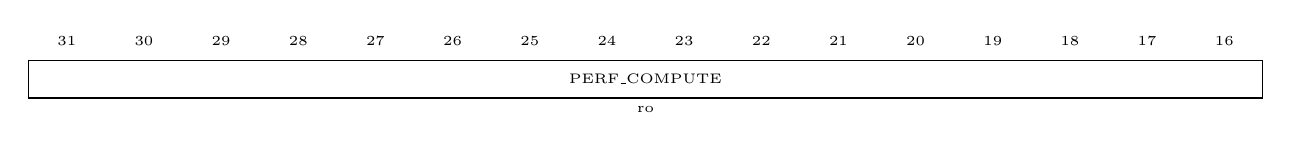
\begin{tikzpicture}[x=0.98cm,y=0.6cm]
\node[font=\tiny] at (0.5,1.2) {31};
\node[font=\tiny] at (1.5,1.2) {30};
\node[font=\tiny] at (2.5,1.2) {29};
\node[font=\tiny] at (3.5,1.2) {28};
\node[font=\tiny] at (4.5,1.2) {27};
\node[font=\tiny] at (5.5,1.2) {26};
\node[font=\tiny] at (6.5,1.2) {25};
\node[font=\tiny] at (7.5,1.2) {24};
\node[font=\tiny] at (8.5,1.2) {23};
\node[font=\tiny] at (9.5,1.2) {22};
\node[font=\tiny] at (10.5,1.2) {21};
\node[font=\tiny] at (11.5,1.2) {20};
\node[font=\tiny] at (12.5,1.2) {19};
\node[font=\tiny] at (13.5,1.2) {18};
\node[font=\tiny] at (14.5,1.2) {17};
\node[font=\tiny] at (15.5,1.2) {16};
\draw (0,0) rectangle (16,0.8);
\node[font=\tiny] at (8.0,0.4) {PERF\_COMPUTE};
\node[font=\tiny] at (8.0,-0.25) {ro};
\end{tikzpicture}
\end{center}
\begin{center}
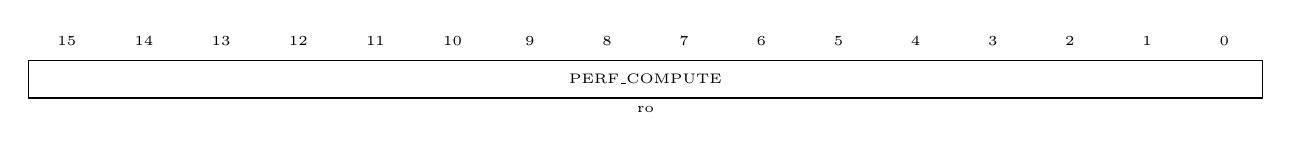
\begin{tikzpicture}[x=0.98cm,y=0.6cm]
\node[font=\tiny] at (0.5,1.2) {15};
\node[font=\tiny] at (1.5,1.2) {14};
\node[font=\tiny] at (2.5,1.2) {13};
\node[font=\tiny] at (3.5,1.2) {12};
\node[font=\tiny] at (4.5,1.2) {11};
\node[font=\tiny] at (5.5,1.2) {10};
\node[font=\tiny] at (6.5,1.2) {9};
\node[font=\tiny] at (7.5,1.2) {8};
\node[font=\tiny] at (8.5,1.2) {7};
\node[font=\tiny] at (9.5,1.2) {6};
\node[font=\tiny] at (10.5,1.2) {5};
\node[font=\tiny] at (11.5,1.2) {4};
\node[font=\tiny] at (12.5,1.2) {3};
\node[font=\tiny] at (13.5,1.2) {2};
\node[font=\tiny] at (14.5,1.2) {1};
\node[font=\tiny] at (15.5,1.2) {0};
\draw (0,0) rectangle (16,0.8);
\node[font=\tiny] at (8.0,0.4) {PERF\_COMPUTE};
\node[font=\tiny] at (8.0,-0.25) {ro};
\end{tikzpicture}
\end{center}
\begin{spectable}{|L{0.09}|L{0.24}|L{0.08}|L{0.15}|L{0.44}|}{Số chu kỳ COMPUTE}{reg:PERF_COMPUTE}{\textbf{Bit} & \textbf{Tên} & \textbf{Kiểu} & \textbf{Giá trị mặc định} & \textbf{Mô tả}}
31:0 & PERF\_COMPUTE & RO & 32'h0 & Số chu kỳ COMPUTE. Xóa khi nhận tác vụ hoặc reset; bão hòa tại 0xFFFF\_FFFF, giữ sau khi kết thúc. \\\hline

\end{spectable}

\subsection{Số chu kỳ STORE\_C (PERF\_STORE)}
Địa chỉ offset: 0x38\par
Giá trị reset: 0x0000\_0000\par
\begin{center}
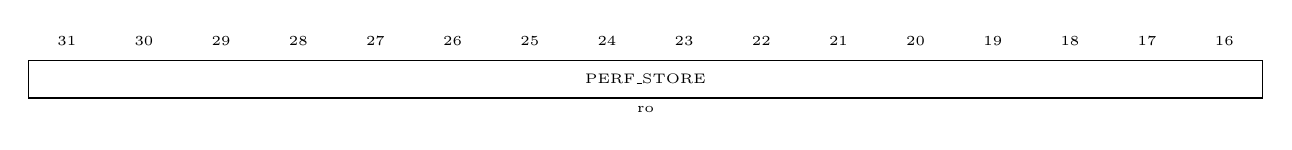
\begin{tikzpicture}[x=0.98cm,y=0.6cm]
\node[font=\tiny] at (0.5,1.2) {31};
\node[font=\tiny] at (1.5,1.2) {30};
\node[font=\tiny] at (2.5,1.2) {29};
\node[font=\tiny] at (3.5,1.2) {28};
\node[font=\tiny] at (4.5,1.2) {27};
\node[font=\tiny] at (5.5,1.2) {26};
\node[font=\tiny] at (6.5,1.2) {25};
\node[font=\tiny] at (7.5,1.2) {24};
\node[font=\tiny] at (8.5,1.2) {23};
\node[font=\tiny] at (9.5,1.2) {22};
\node[font=\tiny] at (10.5,1.2) {21};
\node[font=\tiny] at (11.5,1.2) {20};
\node[font=\tiny] at (12.5,1.2) {19};
\node[font=\tiny] at (13.5,1.2) {18};
\node[font=\tiny] at (14.5,1.2) {17};
\node[font=\tiny] at (15.5,1.2) {16};
\draw (0,0) rectangle (16,0.8);
\node[font=\tiny] at (8.0,0.4) {PERF\_STORE};
\node[font=\tiny] at (8.0,-0.25) {ro};
\end{tikzpicture}
\end{center}
\begin{center}
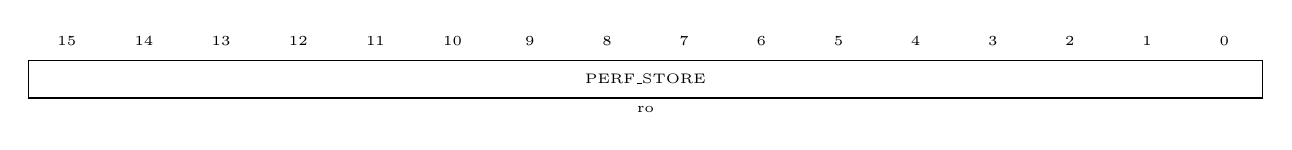
\begin{tikzpicture}[x=0.98cm,y=0.6cm]
\node[font=\tiny] at (0.5,1.2) {15};
\node[font=\tiny] at (1.5,1.2) {14};
\node[font=\tiny] at (2.5,1.2) {13};
\node[font=\tiny] at (3.5,1.2) {12};
\node[font=\tiny] at (4.5,1.2) {11};
\node[font=\tiny] at (5.5,1.2) {10};
\node[font=\tiny] at (6.5,1.2) {9};
\node[font=\tiny] at (7.5,1.2) {8};
\node[font=\tiny] at (8.5,1.2) {7};
\node[font=\tiny] at (9.5,1.2) {6};
\node[font=\tiny] at (10.5,1.2) {5};
\node[font=\tiny] at (11.5,1.2) {4};
\node[font=\tiny] at (12.5,1.2) {3};
\node[font=\tiny] at (13.5,1.2) {2};
\node[font=\tiny] at (14.5,1.2) {1};
\node[font=\tiny] at (15.5,1.2) {0};
\draw (0,0) rectangle (16,0.8);
\node[font=\tiny] at (8.0,0.4) {PERF\_STORE};
\node[font=\tiny] at (8.0,-0.25) {ro};
\end{tikzpicture}
\end{center}
\begin{spectable}{|L{0.09}|L{0.24}|L{0.08}|L{0.15}|L{0.44}|}{Số chu kỳ STORE\_C}{reg:PERF_STORE}{\textbf{Bit} & \textbf{Tên} & \textbf{Kiểu} & \textbf{Giá trị mặc định} & \textbf{Mô tả}}
31:0 & PERF\_STORE & RO & 32'h0 & Số chu kỳ STORE\_C. Xóa khi nhận tác vụ hoặc reset; bão hòa tại 0xFFFF\_FFFF, giữ sau khi kết thúc. \\\hline

\end{spectable}

\subsection{Con trỏ descriptor đầu (DESC\_PTR)}
Địa chỉ offset: 0x40\par
Giá trị reset: 0x0000\_0000\par
\begin{center}
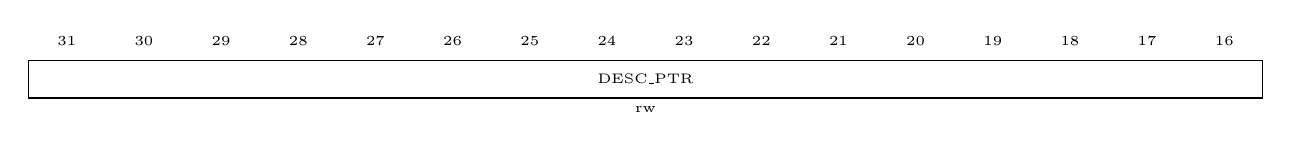
\begin{tikzpicture}[x=0.98cm,y=0.6cm]
\node[font=\tiny] at (0.5,1.2) {31};
\node[font=\tiny] at (1.5,1.2) {30};
\node[font=\tiny] at (2.5,1.2) {29};
\node[font=\tiny] at (3.5,1.2) {28};
\node[font=\tiny] at (4.5,1.2) {27};
\node[font=\tiny] at (5.5,1.2) {26};
\node[font=\tiny] at (6.5,1.2) {25};
\node[font=\tiny] at (7.5,1.2) {24};
\node[font=\tiny] at (8.5,1.2) {23};
\node[font=\tiny] at (9.5,1.2) {22};
\node[font=\tiny] at (10.5,1.2) {21};
\node[font=\tiny] at (11.5,1.2) {20};
\node[font=\tiny] at (12.5,1.2) {19};
\node[font=\tiny] at (13.5,1.2) {18};
\node[font=\tiny] at (14.5,1.2) {17};
\node[font=\tiny] at (15.5,1.2) {16};
\draw (0,0) rectangle (16,0.8);
\node[font=\tiny] at (8.0,0.4) {DESC\_PTR};
\node[font=\tiny] at (8.0,-0.25) {rw};
\end{tikzpicture}
\end{center}
\begin{center}
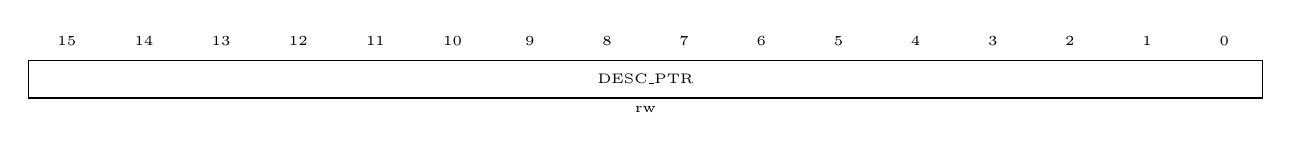
\begin{tikzpicture}[x=0.98cm,y=0.6cm]
\node[font=\tiny] at (0.5,1.2) {15};
\node[font=\tiny] at (1.5,1.2) {14};
\node[font=\tiny] at (2.5,1.2) {13};
\node[font=\tiny] at (3.5,1.2) {12};
\node[font=\tiny] at (4.5,1.2) {11};
\node[font=\tiny] at (5.5,1.2) {10};
\node[font=\tiny] at (6.5,1.2) {9};
\node[font=\tiny] at (7.5,1.2) {8};
\node[font=\tiny] at (8.5,1.2) {7};
\node[font=\tiny] at (9.5,1.2) {6};
\node[font=\tiny] at (10.5,1.2) {5};
\node[font=\tiny] at (11.5,1.2) {4};
\node[font=\tiny] at (12.5,1.2) {3};
\node[font=\tiny] at (13.5,1.2) {2};
\node[font=\tiny] at (14.5,1.2) {1};
\node[font=\tiny] at (15.5,1.2) {0};
\draw (0,0) rectangle (16,0.8);
\node[font=\tiny] at (8.0,0.4) {DESC\_PTR};
\node[font=\tiny] at (8.0,-0.25) {rw};
\end{tikzpicture}
\end{center}
\begin{spectable}{|L{0.09}|L{0.24}|L{0.08}|L{0.15}|L{0.44}|}{Con trỏ descriptor đầu}{reg:DESC_PTR}{\textbf{Bit} & \textbf{Tên} & \textbf{Kiểu} & \textbf{Giá trị mặc định} & \textbf{Mô tả}}
31:0 & DESC\_PTR & RW & 32'h0 & Địa chỉ byte descriptor đầu; căn 64 byte. Khi HAS\_CHAIN = 0: đọc 0, ghi bị bỏ qua. \\\hline

\end{spectable}

\subsection{Địa chỉ descriptor lỗi (ERR\_DESC\_ADDR)}
Địa chỉ offset: 0x44\par
Giá trị reset: 0x0000\_0000\par
\begin{center}
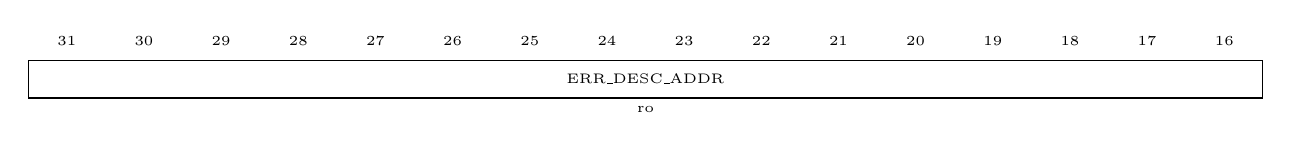
\begin{tikzpicture}[x=0.98cm,y=0.6cm]
\node[font=\tiny] at (0.5,1.2) {31};
\node[font=\tiny] at (1.5,1.2) {30};
\node[font=\tiny] at (2.5,1.2) {29};
\node[font=\tiny] at (3.5,1.2) {28};
\node[font=\tiny] at (4.5,1.2) {27};
\node[font=\tiny] at (5.5,1.2) {26};
\node[font=\tiny] at (6.5,1.2) {25};
\node[font=\tiny] at (7.5,1.2) {24};
\node[font=\tiny] at (8.5,1.2) {23};
\node[font=\tiny] at (9.5,1.2) {22};
\node[font=\tiny] at (10.5,1.2) {21};
\node[font=\tiny] at (11.5,1.2) {20};
\node[font=\tiny] at (12.5,1.2) {19};
\node[font=\tiny] at (13.5,1.2) {18};
\node[font=\tiny] at (14.5,1.2) {17};
\node[font=\tiny] at (15.5,1.2) {16};
\draw (0,0) rectangle (16,0.8);
\node[font=\tiny] at (8.0,0.4) {ERR\_DESC\_ADDR};
\node[font=\tiny] at (8.0,-0.25) {ro};
\end{tikzpicture}
\end{center}
\begin{center}
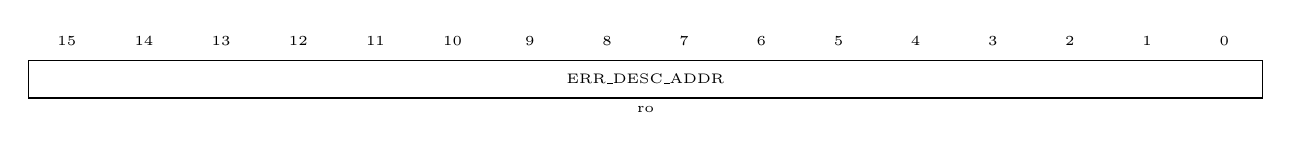
\begin{tikzpicture}[x=0.98cm,y=0.6cm]
\node[font=\tiny] at (0.5,1.2) {15};
\node[font=\tiny] at (1.5,1.2) {14};
\node[font=\tiny] at (2.5,1.2) {13};
\node[font=\tiny] at (3.5,1.2) {12};
\node[font=\tiny] at (4.5,1.2) {11};
\node[font=\tiny] at (5.5,1.2) {10};
\node[font=\tiny] at (6.5,1.2) {9};
\node[font=\tiny] at (7.5,1.2) {8};
\node[font=\tiny] at (8.5,1.2) {7};
\node[font=\tiny] at (9.5,1.2) {6};
\node[font=\tiny] at (10.5,1.2) {5};
\node[font=\tiny] at (11.5,1.2) {4};
\node[font=\tiny] at (12.5,1.2) {3};
\node[font=\tiny] at (13.5,1.2) {2};
\node[font=\tiny] at (14.5,1.2) {1};
\node[font=\tiny] at (15.5,1.2) {0};
\draw (0,0) rectangle (16,0.8);
\node[font=\tiny] at (8.0,0.4) {ERR\_DESC\_ADDR};
\node[font=\tiny] at (8.0,-0.25) {ro};
\end{tikzpicture}
\end{center}
\begin{spectable}{|L{0.09}|L{0.24}|L{0.08}|L{0.15}|L{0.44}|}{Địa chỉ descriptor lỗi}{reg:ERR_DESC_ADDR}{\textbf{Bit} & \textbf{Tên} & \textbf{Kiểu} & \textbf{Giá trị mặc định} & \textbf{Mô tả}}
31:0 & ERR\_DESC\_ADDR & RO & 32'h0 & Địa chỉ descriptor có lỗi sớm nhất theo thứ tự chuỗi. Xóa khi nhận tác vụ/reset; bằng 0 ở chế độ đơn hoặc khi không có chuỗi. \\\hline

\end{spectable}

\subsection{Số descriptor hoàn tất (DESC\_DONE\_CNT)}
Địa chỉ offset: 0x48\par
Giá trị reset: 0x0000\_0000\par
\begin{center}
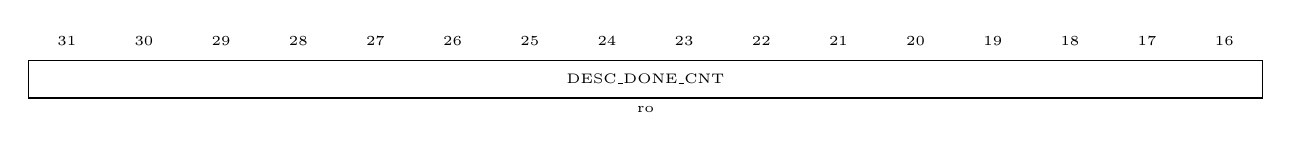
\begin{tikzpicture}[x=0.98cm,y=0.6cm]
\node[font=\tiny] at (0.5,1.2) {31};
\node[font=\tiny] at (1.5,1.2) {30};
\node[font=\tiny] at (2.5,1.2) {29};
\node[font=\tiny] at (3.5,1.2) {28};
\node[font=\tiny] at (4.5,1.2) {27};
\node[font=\tiny] at (5.5,1.2) {26};
\node[font=\tiny] at (6.5,1.2) {25};
\node[font=\tiny] at (7.5,1.2) {24};
\node[font=\tiny] at (8.5,1.2) {23};
\node[font=\tiny] at (9.5,1.2) {22};
\node[font=\tiny] at (10.5,1.2) {21};
\node[font=\tiny] at (11.5,1.2) {20};
\node[font=\tiny] at (12.5,1.2) {19};
\node[font=\tiny] at (13.5,1.2) {18};
\node[font=\tiny] at (14.5,1.2) {17};
\node[font=\tiny] at (15.5,1.2) {16};
\draw (0,0) rectangle (16,0.8);
\node[font=\tiny] at (8.0,0.4) {DESC\_DONE\_CNT};
\node[font=\tiny] at (8.0,-0.25) {ro};
\end{tikzpicture}
\end{center}
\begin{center}
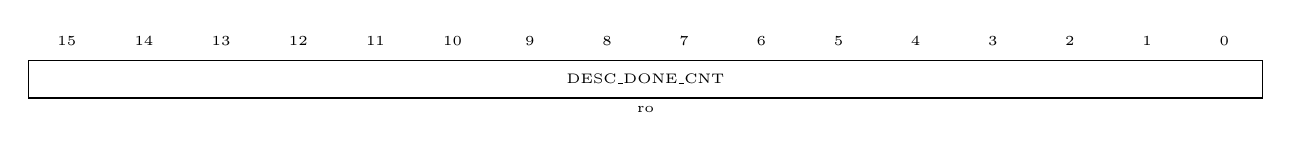
\begin{tikzpicture}[x=0.98cm,y=0.6cm]
\node[font=\tiny] at (0.5,1.2) {15};
\node[font=\tiny] at (1.5,1.2) {14};
\node[font=\tiny] at (2.5,1.2) {13};
\node[font=\tiny] at (3.5,1.2) {12};
\node[font=\tiny] at (4.5,1.2) {11};
\node[font=\tiny] at (5.5,1.2) {10};
\node[font=\tiny] at (6.5,1.2) {9};
\node[font=\tiny] at (7.5,1.2) {8};
\node[font=\tiny] at (8.5,1.2) {7};
\node[font=\tiny] at (9.5,1.2) {6};
\node[font=\tiny] at (10.5,1.2) {5};
\node[font=\tiny] at (11.5,1.2) {4};
\node[font=\tiny] at (12.5,1.2) {3};
\node[font=\tiny] at (13.5,1.2) {2};
\node[font=\tiny] at (14.5,1.2) {1};
\node[font=\tiny] at (15.5,1.2) {0};
\draw (0,0) rectangle (16,0.8);
\node[font=\tiny] at (8.0,0.4) {DESC\_DONE\_CNT};
\node[font=\tiny] at (8.0,-0.25) {ro};
\end{tikzpicture}
\end{center}
\begin{spectable}{|L{0.09}|L{0.24}|L{0.08}|L{0.15}|L{0.44}|}{Số descriptor hoàn tất}{reg:DESC_DONE_CNT}{\textbf{Bit} & \textbf{Tên} & \textbf{Kiểu} & \textbf{Giá trị mặc định} & \textbf{Mô tả}}
31:0 & DESC\_DONE\_CNT & RO & 32'h0 & Tăng khi STORE\_C của descriptor thành công. Xóa khi nhận tác vụ/reset; bằng 0 ở chế độ đơn hoặc khi không có chuỗi. \\\hline

\end{spectable}

\subsection{Mã lỗi}
\begin{spectable}{|L{0.12}|L{0.25}|L{0.63}|}{Mã lỗi \sigc{ERR_CODE} (STATUS[7:4])}{tab:3-2}{\textbf{Giá trị} & \textbf{Ý nghĩa} & \textbf{Khi nào xuất hiện}}
0 & Không lỗi & ERROR = 0 \\\hline

1 & Cấu hình sai & Bản chụp vi phạm điều kiện hợp lệ của thanh ghi; hoặc START và START\_CHAIN cùng được ghi 1 \\\hline

2 & Lỗi AXI khi đọc & LOAD\_A, LOAD\_B hoặc LOAD\_BIAS gặp \sig{rresp} ≠ OKAY hoặc \sig{rlast} sai vị trí \\\hline

3 & Lỗi AXI khi ghi & STORE\_C gặp \sig{bresp} ≠ OKAY \\\hline

4 & Lỗi AXI khi đọc descriptor & Chỉ có với phần bổ sung (mục~\ref{sec:7.2}) \\\hline

5 & Tính năng không có & START\_CHAIN khi phần cứng không có chế độ chuỗi \\\hline

6–15 & Dự trữ & Không bao giờ xuất hiện \\\hline

\end{spectable}

\label{tab:3-3}

\subsection{Yêu cầu thanh ghi}\label{sec:3.2}


\paragraph{Thanh ghi}\label{tab:3-4}
\begin{itemize}
\item Offset, tên, quyền truy cập và giá trị reset theo register map ở trên
\item CTRL[0] START: ghi 1 là yêu cầu bắt đầu tác vụ; bit tự xóa, đọc luôn ra 0; ghi 0 không có tác dụng
\item CTRL[1] SOFT\_RESET: ghi 1 là yêu cầu soft reset (mục~\ref{sec:4.5}); tự xóa
\item CTRL[2] START\_CHAIN: khi \sig{HAS_CHAIN} = 0, lệnh vẫn được chấp nhận như một tác vụ và kết thúc ngay với ERROR, \sig{ERR_CODE} = 5, không truy cập bus
\item Một lần ghi CTRL có SOFT\_RESET = 1: chỉ SOFT\_RESET có hiệu lực. Không có SOFT\_RESET mà START = START\_CHAIN = 1: tác vụ được chấp nhận và kết thúc ngay với \sig{ERR_CODE} = 1
\item STATUS.MODE = 0 với tác vụ START, = 1 với tác vụ START\_CHAIN; giữ giá trị của tác vụ gần nhất. \sig{ERR_CODE} = 0 khi ERROR = 0
\item Thanh ghi R/W được ghi bất kỳ lúc nào, kể cả khi BUSY = 1. Đọc lại trả giá trị CPU đã ghi, không phải bản chụp. Giá trị mới áp dụng từ lần START được chấp nhận tiếp theo
\item Thanh ghi R/W lưu đủ 32 bit, kể cả bit dự trữ, để phát hiện cấu hình có trường dự trữ khác 0. Bit dự trữ của CTRL và STATUS: ghi bị bỏ qua, đọc ra 0. Offset dự trữ: đọc ra 0, ghi bị bỏ qua. Ghi vào thanh ghi chỉ đọc bị bỏ qua
\item \sig{rst_n} đưa mọi thanh ghi về giá trị reset. Soft reset giữ nguyên các thanh ghi R/W; xóa STATUS và \sig{PERF_*}
\item \sig{PERF_*} về 0 ở chu kỳ START được chấp nhận, đếm trong lúc BUSY = 1, dừng khi tác vụ kết thúc, bão hòa ở 0xFFFF\_FFFF
\item Bản chụp cấu hình gồm \sig{MATRIX_DIM}, ba \sig{BASE_ADDR_*}, \sig{POST_CTRL}, \sig{BIAS_ADDR}, \sig{QUANT_M0}, \sig{QUANT_SHIFT}; lấy ở chu kỳ START được chấp nhận và giữ ổn định tới hết tác vụ
\item Cấu hình hợp lệ khi và chỉ khi: M, N, K trong miền 1 ≤ M ≤ 32 và N, K thuộc \{4, 8, …, 32\}; \sig{MATRIX_DIM[31:24]} = 0; \sig{BASE_ADDR_IN}, \sig{BASE_ADDR_WEIGHT}, \sig{BASE_ADDR_OUT} có bit [1:0] = 0; \sig{POST_CTRL[31:2]} = 0; \sig{RELU_EN} = 1 kéo theo \sig{POST_EN} = 1; nếu \sig{POST_EN} = 1 thì \sig{BIAS_ADDR[1:0]} = 0 và \sig{QUANT_SHIFT[31:5]} = 0. Khi \sig{POST_EN} = 0, \sig{BIAS_ADDR}, \sig{QUANT_M0}, \sig{QUANT_SHIFT} bị bỏ qua
\end{itemize}


\subsection{Ngữ nghĩa tác vụ}\label{sec:3.3}


\paragraph{Tác vụ}\label{tab:3-5}
\begin{itemize}
\item START chỉ được chấp nhận nếu BUSY = 0 tại chu kỳ Register File thực hiện lệnh ghi CTRL. START khi BUSY = 1 bị bỏ qua, không đổi trạng thái, không báo lỗi
\item Ngay chu kỳ chấp nhận: chụp cấu hình ; xóa DONE, ERROR, \sig{ERR_CODE}, \sig{PERF_*}; đặt MODE. BUSY = 1 từ chu kỳ kế tiếp
\item Register File phát \sig{start_pulse} và chụp cấu hình trước khi trả phản hồi B cho lệnh ghi CTRL; mọi lần đọc STATUS sau khi lệnh ghi hoàn tất đều thấy tác vụ mới
\item DONE = 1 chỉ khi STORE\_C đã nhận phản hồi B cuối cùng là OKAY, tức toàn bộ kết quả đã nằm trong DRAM
\item ERROR = 1 khi gặp một lỗi đã liệt kê ở trên; sau lỗi không pha mới nào được bắt đầu; nội dung vùng đích trong DRAM không xác định
\item BUSY về 0 ở đúng cạnh clock mà DONE hoặc ERROR được đặt. Sau khi chấp nhận và cho tới tác vụ kế tiếp hoặc soft reset, mọi lần đọc STATUS thấy đúng một trong ba bit BUSY, DONE, ERROR bằng 1
\item DONE và ERROR giữ giá trị (sticky); chỉ bị xóa khi tác vụ mới được chấp nhận, khi soft reset hoặc khi \sig{rst_n}
\item Sau DONE hoặc ERROR, firmware được phép ghi START ngay, không cần soft reset
\item Tín hiệu “xong” nội bộ (xong một lệnh DMA, \sig{pe_done}) không hiện ra cho CPU; chỉ STATUS.DONE báo toàn bộ tác vụ xong
\end{itemize}


\subsection{Quy tắc cho firmware}\label{sec:3.4}


\paragraph{Firmware}\label{tab:3-6}
\begin{itemize}
\item Trước lệnh ghi START, firmware thực hiện \sig{fence rw,rw}, để mọi lệnh ghi A, B, bias vào DRAM đến trước lệnh MMIO
\item Firmware chờ bằng polling cho tới khi DONE hoặc ERROR bằng 1, rồi thực hiện \sig{fence rw,rw} trước khi đọc kết quả
\item Đường DMA được giả định nhất quán cache với CPU. Nếu hệ thống tích hợp không bảo đảm điều đó, firmware phải flush dòng cache của A, B, bias trước START và hủy dòng cache của vùng đích sau DONE
\item Firmware không ghi vào vùng DRAM của tác vụ đang chạy
\end{itemize}


\begin{Verbatim}[frame=leftline,framerule=2pt,rulecolor=\color{brand},xleftmargin=6pt,samepage=true]
#define GEMM_BASE  0x60000000u
#define REG(off)   (*(volatile uint32_t *)(GEMM_BASE + (off)))
#define ST_DONE    (1u << 0)
#define ST_ERROR   (1u << 2)

int gemm_run(uint32_t a, uint32_t b, uint32_t c, uint32_t M, uint32_t N,
             uint32_t K, int post, int relu, uint32_t bias,
             int32_t m0, uint32_t sh) {
    REG(0x08) = (K << 16) | (N << 8) | M;     /* MATRIX_DIM   */
    REG(0x0C) = a;  REG(0x10) = b;  REG(0x14) = c;
    REG(0x18) = (post ? 1u : 0u) | (relu ? 2u : 0u);
    REG(0x1C) = bias;  REG(0x20) = (uint32_t)m0;  REG(0x24) = sh;
    asm volatile ("fence rw,rw");             /* (Trước lệnh ghi START, firmware thực hiện \sig{fence rw,rw}, để mọi lệnh ghi A, B, bias vào DRAM đến trước lệnh MMIO ) */
    REG(0x00) = 1u;                           /* START */
    uint32_t s;
    do { s = REG(0x04); } while (!(s & (ST_DONE | ST_ERROR)));
    asm volatile ("fence rw,rw");             /* (Firmware chờ bằng polling cho tới khi DONE hoặc ERROR bằng 1, rồi thực hiện \sig{fence rw,rw} trước khi đọc kết quả ) */
    return (s & ST_ERROR) ? (int)((s >> 4) & 0xFu) : 0;
}
\end{Verbatim}

% Mục 2 — Mô tả chức năng và dữ liệu
